\documentclass[reprint,english,notitlepage,nofootinbib]{revtex4-1}  % defines the basic parameters of the document

% if you want a single-column, remove reprint

% allows special characters (including æøå)
\usepackage[utf8]{inputenc}
\usepackage[english]{babel}

%% note that you may need to download some of these packages manually, it depends on your setup.
%% I recommend downloading TeXMaker, because it includes a large library of the most common packages.

\usepackage{physics,amssymb}  % mathematical symbols (physics imports amsmath)
\numberwithin{equation}{section}
\def\thesection{\arabic{section}}

\usepackage{graphicx}         % include graphics such as plots
\graphicspath{{figs/}} %Setting the graphicspath

\usepackage{xcolor}           % set colors
\usepackage{hyperref}         % automagic cross-referencing (this is GODLIKE)
\usepackage{tikz}             % draw figures manually
\usepackage{listings}         % display code
\usepackage{subfigure}        % imports a lot of cool and useful figure commands

% defines the color of hyperref objects
% Blending two colors:  blue!80!black  =  80% blue and 20% black
\hypersetup{ % this is just my personal choice, feel free to change things
    colorlinks,
    linkcolor={red!50!black},
    citecolor={blue!50!black},
    urlcolor={blue!80!black}}

%% Defines the style of the programming listing
%% This is actually my personal template, go ahead and change stuff if you want
\lstset{ %
	inputpath=,
	backgroundcolor=\color{white!88!black},
	basicstyle={\ttfamily\scriptsize},
	commentstyle=\color{magenta},
	language=Python,
	morekeywords={True,False},
	tabsize=4,
	stringstyle=\color{green!55!black},
	frame=single,
	keywordstyle=\color{blue},
	showstringspaces=false,
	columns=fullflexible,
	keepspaces=true}


%% USEFUL LINKS:
%%
%%   UiO LaTeX guides:        https://www.mn.uio.no/ifi/tjenester/it/hjelp/latex/
%%   mathematics:             https://en.wikibooks.org/wiki/LaTeX/Mathematics

%%   PHYSICS !                https://mirror.hmc.edu/ctan/macros/latex/contrib/physics/physics.pdf

%%   the basics of Tikz:       https://en.wikibooks.org/wiki/LaTeX/PGF/TikZ
%%   all the colors!:          https://en.wikibooks.org/wiki/LaTeX/Colors
%%   how to draw tables:       https://en.wikibooks.org/wiki/LaTeX/Tables
%%   code listing styles:      https://en.wikibooks.org/wiki/LaTeX/Source_Code_Listings
%%   \includegraphics          https://en.wikibooks.org/wiki/LaTeX/Importing_Graphics
%%   learn more about figures  https://en.wikibooks.org/wiki/LaTeX/Floats,_Figures_and_Captions
%%   automagic bibliography:   https://en.wikibooks.org/wiki/LaTeX/Bibliography_Management  (this one is kinda difficult the first time)
%%   REVTeX Guide:             http://www.physics.csbsju.edu/370/papers/Journal_Style_Manuals/auguide4-1.pdf
%%
%%   (this document is of class "revtex4-1", the REVTeX Guide explains how the class works)


%% CREATING THE .pdf FILE USING LINUX IN THE TERMINAL
%%
%% [terminal]$ pdflatex template.tex
%%
%% Run the command twice, always.
%% If you want to use \footnote, you need to run these commands (IN THIS SPECIFIC ORDER)
%%
%% [terminal]$ pdflatex template.tex
%% [terminal]$ bibtex template
%% [terminal]$ pdflatex template.tex
%% [terminal]$ pdflatex template.tex
%%
%% Don't ask me why, I don't know.

\begin{document}
\title{AST3220 - Project 1}   % self-explanatory
\date{\today}                             % self-explanatory
\noaffiliation                            % ignore this
\begin{abstract}                          % marks the beginning of the abstract
\end{abstract}                            % marks the end of the abstract
\maketitle                                % creates the title, author, date & abstract

% the fundamental components of scientific reports:
The scalar field has energy density and pressure
\begin{align}
	\rho_{\phi} = \frac{1}{2} \dot{\phi}^2 + V(\phi) \label{eq:density} \\
	   p_{\phi} = \frac{1}{2} \dot{\phi}^2 - V(\phi) \label{eq:pressure}
\end{align}
\section{Problem 1}
Assuming the quintessence field follows the continuity equation
\begin{align}
	\dot{\rho}_{\phi} &= -3H\left(\rho_{\phi} + p_{\phi}\right) \\
										&= -3\frac{\dot{a}}{a}\left(1 + w_{\phi}\right)\rho_{\phi}
\end{align}
we can begin solving for the density by separating the variables:
\begin{align}\label{eq:drho}
	\frac{1}{\rho_{\phi}} d\rho_{\phi} = -\frac{3}{a}\left(1+w_{\phi}\right)da
\end{align}
We then rewrite $a(t)$ in terms of the cosmological redshift of light emitted at some point $t$ in the past:
\begin{align}
	1+z = \frac{a_0}{a(t)} \ &\Rightarrow a(t) = \frac{a_0}{1+z} \\
													 &\Rightarrow da  = -\frac{a_0}{(1+z)^2}dz
\end{align}
Inserting these into eq. \ref{eq:drho} and integrating from some time $t$ to
today, we get:
\begin{align}
	\int^{\rho_{\phi0}}_{\rho_{\phi}} d\rho_{\phi} \frac{1}{\rho_{\phi}}
	= \int^{0}_z dz' \frac{3[1+w_\phi (z')]}{(1+z')}
\end{align}
We then flip the integration limits on both sides, canceling the negatives.
Computing the left hand integral and solving for $\rho_\phi$ we then get the solution
\begin{align}
	\rho_\phi(z) = \rho_{\phi 0} \
	\mathrm{exp}\left\{ \int^{z}_0 dz' \frac{3[1+w_\phi (z')]}{(1+z')}\right\}
\end{align}

\section{Problem 2}
Inserting equations for the density (\ref{eq:density}) and pressure
(\ref{eq:pressure}) of the scalar field into the continuity equation we get
\begin{align}
	\dot{\rho}_\phi &= -3H\left(\rho_\phi + p_\phi \left) \\
									&= -3H\dot{\phi}^2
\end{align}
We can also find an expression for $\dot{\rho}_\phi$ directly, by taking the
time derivative of equation (\ref{eq:density}):
\begin{align}
	\dot{\rho}_\phi &= \frac{d}{dt}\left(\frac{1}{2} \dot{\phi}^2 + V(\phi) \right)\\
					  			&= \dot{\phi} \ddot{\phi} + {V}'(\phi) \dot{\phi}
\end{align}
Equating the two expressions, we get the differential equation:
\begin{align}
	\ddot{\phi}\dot{\phi}  + 3H\dot{\phi}^2 + {V}'(\phi) \dot{\phi} = 0
\end{align}
Ignoring the boring case of a static $\phi(t)=\phi_0$, we have $\dot{\phi} \neq0$.
The equation can then be reduced to:
\begin{align}
	\ddot{\phi} + 3H\dot{\phi} + {V}'(\phi) = 0 \label{eq:phi_ddot}
\end{align}

\section{Problem 3}
Taking the time-derivative of the Hubble parameter
\begin{align}
	\dot{H} = \frac{d}{dt}\left(\frac{\dot{a}}{a}\right) = \frac{\ddot{a}}{a} - \left(\frac{\dot{a}}{a}\right)^2 \label{eq:Hdot}
\end{align}
we recognize both terms on the right hand side from the Friedmann equations. For a flat ($k=0$) universe the Friedmann equations read
\begin{align}
	\left(\frac{\dot{a}}{a}\right)^2 &= \frac{\kappa^2}{3}\rho \\
	\frac{\ddot{a}}{a}		&= -\frac{\kappa^2}{6}\left(\rho + 3p \right)
\end{align}
Where we have defined $\kappa^2 = 8\pi G$. For a universe with matter, radiation
and quintessence we have
\begin{align}
	\rho &= \rho_m + \rho_r + \rho_\phi \\
	p    &= p_m + p_r + p_\phi \\
         &= w_{r}\rho_r + p_{\phi}
\end{align}
Since the equation of state parameter for non-relativistic matter is $w_{m} = 0$.
Inserting the Friedmann equations into (\ref{eq:Hdot}), and using $\rho_{\phi} + p_{\phi} = \dot{\phi}$, we then
get:
\begin{align}
	\dot{H} &= -\frac{\kappa^2}{6}\left(\rho + 3p \right) - \frac{\kappa^2}{3}\rho \\
					&= -\frac{\kappa^2}{2} \left[\rho + p \right] \\
					&= -\frac{\kappa^2}{2} \left[ \rho_m + \rho_r + \rho_r w_r + \rho_{\phi} + p_{\phi}\right]\\
					&= -\frac{\kappa^2}{2} \left[ \rho_m + \rho_r(1+w_r) + \dot{\phi}\right]
\end{align}

\section{Problem 4}\label{sec:4}
Introducing the dimensionless variables
\begin{align}
	x_1 = \frac{\kappa \dot{\phi}}{\sqrt{6}H} \\
	x_2 = \frac{\kappa \sqrt{V}}{\sqrt{3}H} \\
	x_3 = \frac{\kappa \sqrt{\rho_r}}{\sqrt{3}H} \\
\end{align}
we notice their squares can be rewritten them in terms of the critical density
$\rho_c = \frac{3H^2}{\kappa^2}$:
\begin{align}
	x_1^2 &= \frac{\frac{1}{2}\dot{\phi}^2}{\rho_c} \label{eq:x1} \\
	x_2^2 &= \frac{V}{\rho_c} \label{eq:x2} \\
	x_3^2 &= \frac{\rho_r}{\rho_c} \label{eq:x3} \\
\end{align}
Using the definition $\Omega_i = \frac{\rho_i}{\rho_c}$, the density parameters for quintessence and radiation can be expressed as:
\begin{align}
	\Omega_\phi &= \frac{\frac{1}{2}\dot{\phi} + V}{\rho_c} = x_1^2 + x_2^2 \\
	\Omega_r &= \frac{\rho_r}{\rho_c} = x_3^2
\end{align}
Lastly we want to find an expression for the density parameter for
mass. We accomplish this by taking advantage of our model being
spatially flat, meaning $\frac{\rho}{\rho_c} = 1$. Expanding $\rho$
we get
\begin{align}
	1 &= \frac{\rho_\phi + \rho_r + \rho_m}{\rho_c} \\
		&= \Omega_\phi + \Omega_r + \Omega_m
\end{align}
Which we can solve for $\Omega_m$:
\begin{align}
	\Omega_m &= 1 - \Omega_\phi - \Omega_m \\
					 &= 1 - x_1^2 - x_2^2 - x_3^2
\end{align}

\section{Problem 5}
Next we want to rewrite equation (\ref{eq:Hdot}) in terms of the dimensionless
variables. Using the definitions of the density parameters and the dimensionless
variables we get:
\begin{align}
	\dot{H} &= -\frac{\kappa^2}{2} \left[ \rho_m + \rho_r(1+w_r) + \dot{\phi}\right] \\
					&= -\frac{\kappa^2 \rho_c}{2}\left[\Omega_m + \Omega_r(1+w_r) + 2\Omega_\phi -2x_2^2\right] \\
					&= -\frac{3H^2}{2}\left[1 + x_1^2 -x_2^2 -x_3^2 + x_3^2(1+w_r)\right]
\end{align}
Simplyfing and inserting the radiation equation of state parameter $w_r = 1/3$,
we get:
\begin{align}
	\frac{\dot{H}}{H^2} &= -\frac{1}{2}\left[3+3x_1^2 -3x_2^2 + x_3^2\right] \label{eq:H_dim}
\end{align}

\section{Problem 6}
\subsection{Equation of motion for $x_1$}
Using the product rule:
\begin{align}
	\frac{dx_1}{dN} &= \frac{1}{H}\frac{dx_1}{dt} \\
	&= \frac{\kappa}{\sqrt{6}H}\frac{d}{dt}\left(\frac{\dot{\phi}}{H}\right)\\
	&= \frac{\kappa\ddot{\phi}}{\sqrt{6}H^2} - \frac{\kappa\dot{\phi}}{\sqrt{6}H}\frac{\dot{H}}{H^2}
\end{align}
From equation (\ref{eq:phi_ddot}) we have $\ddot{\phi}=-3H\dot{\phi}-{V}$.
Inserting for $\ddot{\phi}$ and $\dot{H}/H^2$ (eq. \ref{eq:H_dim}) we then get:
\begin{align}
	\frac{dx_1}{dN} &= -\frac{3\kappa\dot{\phi}}{\sqrt{6}H} - \frac{\kappa V'}{\sqrt{6}H}
										+ \frac{\kappa\dot{\phi}}{\sqrt{6}H}\frac{\dot{H}}{H} \\
									&= -3x_1	 + \frac{\sqrt{6}}{2}\lambda x_2^2
										+ \frac{1}{2}x_1(3+3x_1 - 3x_2^2 + 3x_3^3)
\end{align}
Where we have defined $\lambda$ as
\begin{align}
	\lambda = -\frac{V'}{\kappa V}
\end{align}

\subsection{Equation of motion for $x_2$}
The equation for $x_2$ is found in a similar manner, we get:
\begin{align}
	\frac{dx_2}{dN} &= \frac{\kappa}{\sqrt{3}H}\frac{d}{dt}\left(\frac{\sqrt{V}}{H}\right)\\
									&= \frac{\kappa}{\sqrt{3}H}\left(\frac{1}{2}\frac{V'\dot{\phi}}
									{\sqrt{\phi}H}-\sqrt{V}\frac{\dot{H}}{H^2}\right) \\
									&=\frac{\sqrt{6}}{2}\frac{V'}{\kappa V}\frac{\kappa \sqrt{V}}{\sqrt{3}H}
										\frac{\kappa\dot{\phi}}{\sqrt{6}H} - \frac{\kappa\sqrt{V}}{\sqrt{3}H}
										\frac{\dot{H}}{H^2} \\
									&=\frac{\sqrt{6}}{2}\lambda x_1 x_2 + \frac{1}{2}x_2
									(3+3x_1 - 3x_2^2 + 3x_3^3)
\end{align}
\subsection{Equation of motion for $x_3$}
Similarly, for $x_3$:

\begin{align}
	\frac{dx_3}{dN} &= \frac{\kappa}{\sqrt{3}H}\frac{d}{dt}\left(\frac{\sqrt{\rho_r}}{H}\right)\\
									&= \frac{\kappa}{\sqrt{3}H}\left(\frac{1}{2}\frac{\dot{\rho}_r}
									{\sqrt{\rho_r}H} - \sqrt{\rho_r}\frac{\dot{H}}{H^2}\right)\\
\end{align}
Where $\dot{\rho}_r$ is given by the continuity equation:
\begin{align}
	\dot{\rho}_r &= -3 H (1 + w_r)\rho_r \\
							 &= -4 H\rho_r
\end{align}
Where we used that $w_r=1/3$. Inserting the expressions for $\dot{\rho}_r$ and
$\dot{H}/H^2$ we finally get:
\begin{align}
	\frac{dx_3}{dN} &=-2x_3 + \frac{1}{2}x_3\left(3+3x_1 - 3x_2^2 + 3x_3^3\right)
\end{align}

\section{Problem 7}
Rewriting the expression for $\lambda$ as a differential equation for V, we get:
\begin{align}
	V' + \kappa \lambda V = 0
\end{align}
For a constant $\lambda$ this has the solution
\begin{align}
	V = V_0 e^{-\kappa\lambda\phi}
\end{align}
We can then find the value of $\Gamma$ by simple differentiation:
\begin{align}
	\Gamma &= \frac{V V''}{(V')^2} \\
				 &= \frac{\kappa^2\lambda^2 V^2}{(-\kappa\lambda)^2 V^2} \\
				 &= 1
\end{align}
\section{Problem 8}
For a non-constant $\lambda$ we differentiate $V'V^{-1}$ using the product rule
and chain rule. Massaging the equation a bit, we then get:
\begin{align}
	\frac{d\lambda}{dN} &= -\frac{1}{\kappa H}\frac{d}{dt}\left( \frac{V'}{V}\right) \\
											&= -\frac{1}{\kappa H}\left(\frac{V''}{V}\dot{\phi} -  \frac{(V')^2}{V^2}\dot{\phi}\right) \\
											&= -\frac{\kappa\dot{\phi}}{\sqrt{6}H}\frac{\sqrt{6}}{\kappa^2}
											\left(\frac{V''}{V} - \frac{(V')^2}{V^2}\right) \\
											&= -x_{1}\sqrt{6}\left(\frac{V'}{\kappa V}\right)^2
													\left(\frac{V V''}{(V')^2} - 1 \right) \\
											&= - \sqrt{6} \lambda^2 (\Gamma - 1) x_1
\end{align}
\section{Problem 9}
%After being algebraically harassed, we have at last amassed the tools to numerically blast these equations off the jiggermast and into the past.
At long last, we have amassed, after being algebraically harassed, the tools to
numerically unsurpassed blast these equations off the
jiggermast\footnote{\textbf{Jiggermast - noun}: Any small mast on a sailing vessel;
especially the mizzenmast of a yawl.}.
\\ \\
We note that we can also express the equation of state parameter for
quintessence in terms of the dimensionless variables:
\begin{align}
		w_\phi = \frac{x_1^2 - x_2^2}{x_1^2 + x_2^2}
\end{align}
We can then find both the density parameters (using our results from Problem
\ref{sec:4}) and the equation of state parameters by
integrating the equations of motion of the dimensionless variables numerically.
The density parameters plotted against redshift can be found in Figure
(\ref{fig:omegas}), and the equations of state can be seen in Figure (\ref{fig:eos}).
\\ \\
The density parameters match quite well with what we expect; the early universe
is radiation-dominated, while the universe today is governed primarily by
quintessence ("dark energy"), with smaller contributions from ordinary matter.
\\
\begin{figure}[h!]
	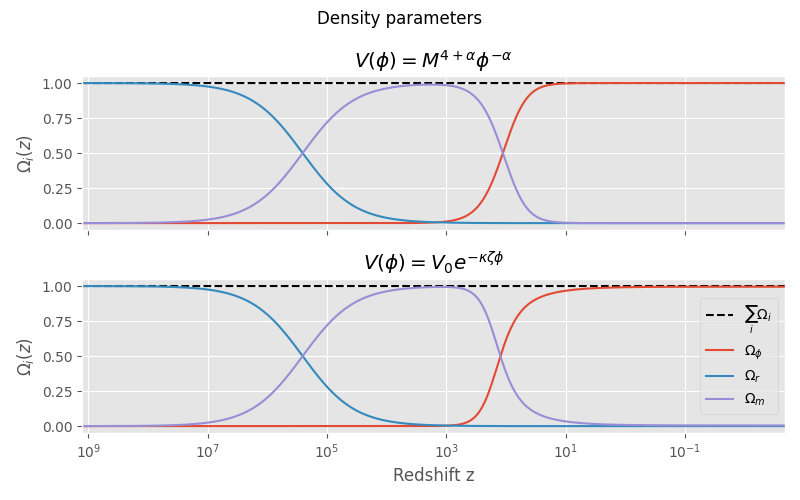
\includegraphics[scale=0.4]{density_parameters.png}
	\caption{Density parameters for quintessence models using a power law potential
	(top) and an exponential potential (bottom), plotted against redshift. The sum
	of all density parameters (which should sum to $1$) is plotted as a quality
	control.}
	\label{fig:omegas}
\end{figure}


\begin{figure}[h!]
	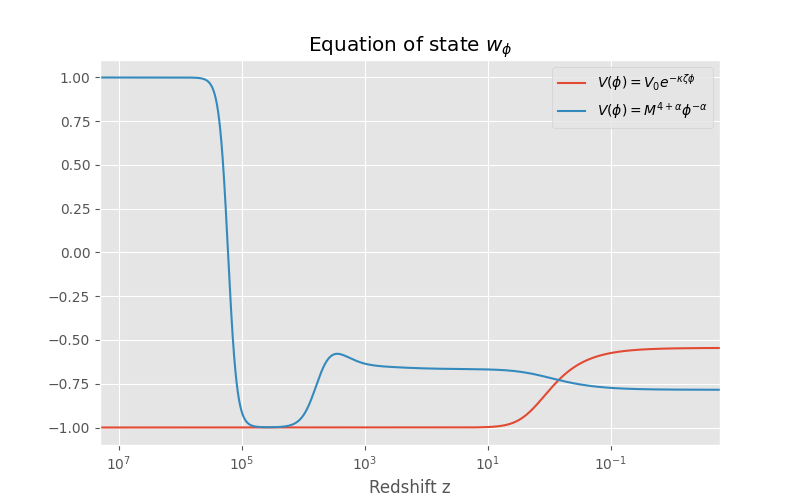
\includegraphics[scale=0.45]{eos.png}
	\caption{Equation of state for quintessence models using a power law potential
	and an exponential potential, plotted against redshift.}
	\label{fig:eos}
\end{figure}

\section{Problem 10}
\subsection{Quintessence models}
We know that the dimensionless Hubble parameter for the quintessence model can
be weritten
\begin{align}\label{eq:HH0}
	\frac{H^2}{H_0^2} = \left[ \Omega_{m0}(1+z)^3 + \Omega_{r0}(1+z)^4
											+ \Omega_{\phi 0}e^{I(z)} \right]
\end{align}
Where $I(z)$ is the integral
\begin{align}
	I(z) = \int_0^z dz' \frac{3[1+w_\phi(z')]}{(1+z')}
\end{align}
Which can be rewritten in terms of the dimensionless variable $N=-\ln(1+z)$.
Using $dz = -(1+z)\ dN$, we get:
\begin{align}
	I(N) &= \int^N_0 dN' (1+z')\frac{3[1 + w_\phi(N')]}{(1+z')} \\
			 &= -3\int^0_N dN' [1+w_\phi(N')]
\end{align}
Inserting this into Eq. (\ref{eq:HH0}), as well as substituting
$(1+z)=e^{-N}$, we get:
\begin{align}
	\frac{H^2}{H_0^2} = \left[ \Omega_{m0}e^{-3N} + \Omega_{r0}e^{-4N}
											+ \Omega_{\phi 0}e^{-I(N)} \right]
\end{align}
Which we evaluate numerically.

\subsection{$\Lambda$CDM model}
For the $\Lambda$CDM model, we use the formula
\begin{align}
	\frac{H^2}{H^2_0} = \Omega_{m0}(1+z)^3 + (1-\Omega_{m0})
\end{align}
The dimensionless Hubble parameters for both quintessence models and the
$\Lambda$CDM model are plotted in Figure (\ref{fig:hubble}). The most surprising
result here is probably that the two quintessence models seem to have such identical
Hubble parameters, in spite of their equations of state parameters being quite different.
We also see that the quintessence models match $\Lambda$CDM quite well for low
redshift, which is a good sign. They do however start deviatiing noticably for
redshift $z\sim10^4$ and greater.

\begin{figure}[h!]
	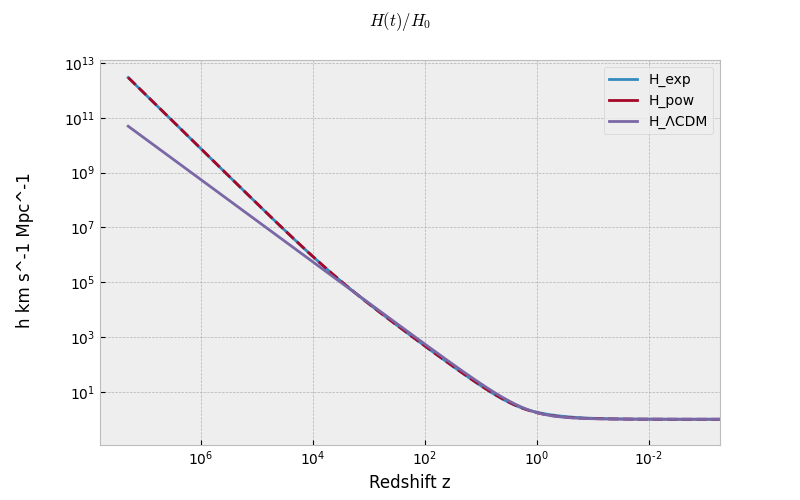
\includegraphics[scale=0.4]{Hubble_param.png}
	\caption{Hubble parameter for both quintessence models and the ΛCDM model plotted
	against redshift.}
	\label{fig:hubble}
\end{figure}

\section{Problem 11}
We calculate the dimensionless age by evaluating the integral
\begin{align}
    H_{0}t_{0} = \int_{0}^{\infty} \frac{dz}{(1+z)H/H_{0}}
\end{align}
Once again substituting in the dimensionless variable $N = -\ln(1+z)$, using
$dz = -(1+z)\ dN$, the integral becomes:
\begin{align}
    H_{0}t_{0} = \int_{-\infty}^{0} \frac{dN}{H/H_{0}}
\end{align}
Approximating this by integrating over the finite arrays
of $H/H_{0}$ we get the dimensionless times in Table
(\ref{tab:H0t0})
\begin{table}
	\begin{tabular}{|l|r|}
\hline
 Model   &     $H_0t_0$ \\
\hline
 V_{exp}(z)     & 0.973745 \\
 V_{pow}(z) & 0.994003 \\
 ΛCDM       & 0.964101 \\
\hline
\end{tabular}
	\caption{The dimensionless age of both quintessence models and the ΛCDM model.}
	\label{tab:H0t0}
\end{table}

\section{Problem 12}
For $k=0$, the luminosity distance as a function of redshift can be written
\begin{align}
    d_{L}(z) = \frac{c(1+z)}{H_{0}} \int_{0}^{z}
    \frac{dz'}{H(z')/H_{0}}
\end{align}
such that the dimensionless becomes:
\begin{align}
    \frac{H_{0}d_{L}}{c} = (1+z) \int_{0}^{z}
    \frac{dz'}{H(z')/H_{0}}
\end{align}
Plotting these for $0\leq z \leq 2$ in both quintessence
models and the $\lambda$CDM model we get the results
shown in figure \ref{fig:lumdistance}

\begin{figure}[h!]
	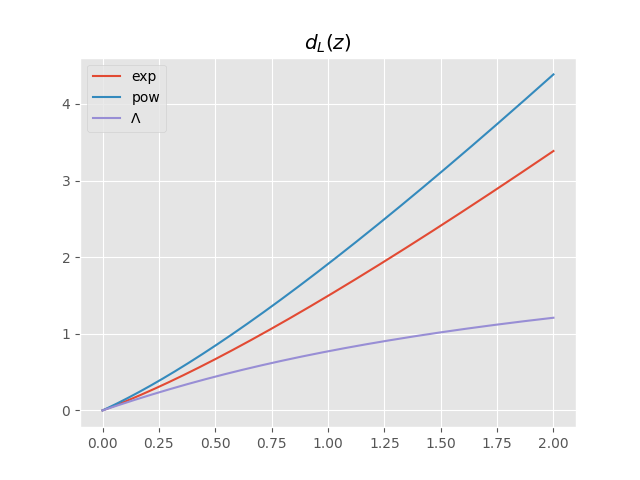
\includegraphics[scale=0.4]{lum_distance.png}
	\caption{The dimensionless luminosity distance for the two quintessence models
	 and the ΛCDM model, plotted against redshift.}
	\label{fig:lumdistance}
\end{figure}

\section{Problem 13}
Calculating $\chi^2$ for the quintessence models, we get
the values shown in Table (\ref{tab:chisquare_quintessence}).
We see that the exponential potential displays a slightly
lower value for $\chi^2$.

\begin{table}
	\begin{tabular}{|l|r|}
\hline
 Potential   &   $\chi^2$  \\
\hline
 Exponential & 1.252e+06   \\
 Power law   & 1.29827e+06 \\
\hline
\end{tabular}
	\caption{}
	\label{tab:chisquare_quintessence}
\end{table}

\section{Problem 14}
To determine the optimal value for $\Omega_{m0}$ we
calculate $\chi^2$ for values in the range $[0,1]$.
With a resolution of $10000$ points, we get the optimal
value
\begin{align}
    \Omega_{m0} \approx 0.2989
\end{align}
with $\chi^2 = 29.74$. (5 orders of magnitude below than the quintessence
models!)

\begin{acknowledgments}  % if you disagree with the spelling, blame Americans
I would like to give a huge thanks to Fysikkforeningen for the
Bunyanesque\footnote{\textbf{Bunyanesque, adjective}: of immense size or stature, as ascribed to Paul Bunyan or to the other characters, exploits, etc., in the legends about him. \\ \\
(Paul Bunyan is a giant lumberjack and folk hero in American and Canadian folklore) } amount of coffee they have supplied me with.
\end{acknowledgments}


%% When it comes to the bibliography I personally generate it using BibLaTeX. (see the link above if you're interested)
%% You're obviously allowed to create the references section however you like.
%% I'll keep it simple here.
\section*{References}  % the asterisk (*) after \section makes the section numbering go away
\begin{itemize}
\item[-]Reference 1
\end{itemize}

\newpage
%% if you want to include an appendix, this is how you do it
\appendix
\section{Name of appendix}
This will be the body of the appendix.
%% all \section commands following \appendix are automatically taken as appendices

%% Note that \label{appendix} command on line 115. What this does is setup a reference point for LaTeX that you can
%% access wherever you want using \ref{appendix}.
%% You can place labels on most environments such as equations, figures, tables, etc.


%% If you want to include figure:
%\includegraphics[scale=1.0]{filename}
%% check https://en.wikibooks.org/wiki/LaTeX/Importing_Graphics if you want to know more

\end{document}
